Pierwszym rozwiązaniem jest skorzystanie z automatycznej, interaktywnej metody  strojenia regulatorów PID dla systemów SISO. Dostęp do niej uzyskuje się poprzez umieszczenie w modelu Simulink bloczka PID, a następnie wybranie opcji Tune widocznej przy parametrach regulatora.
Można również skorzystać z komendy

\textit{pidTuner(sys,type)}.

\begin{figure}[H]
	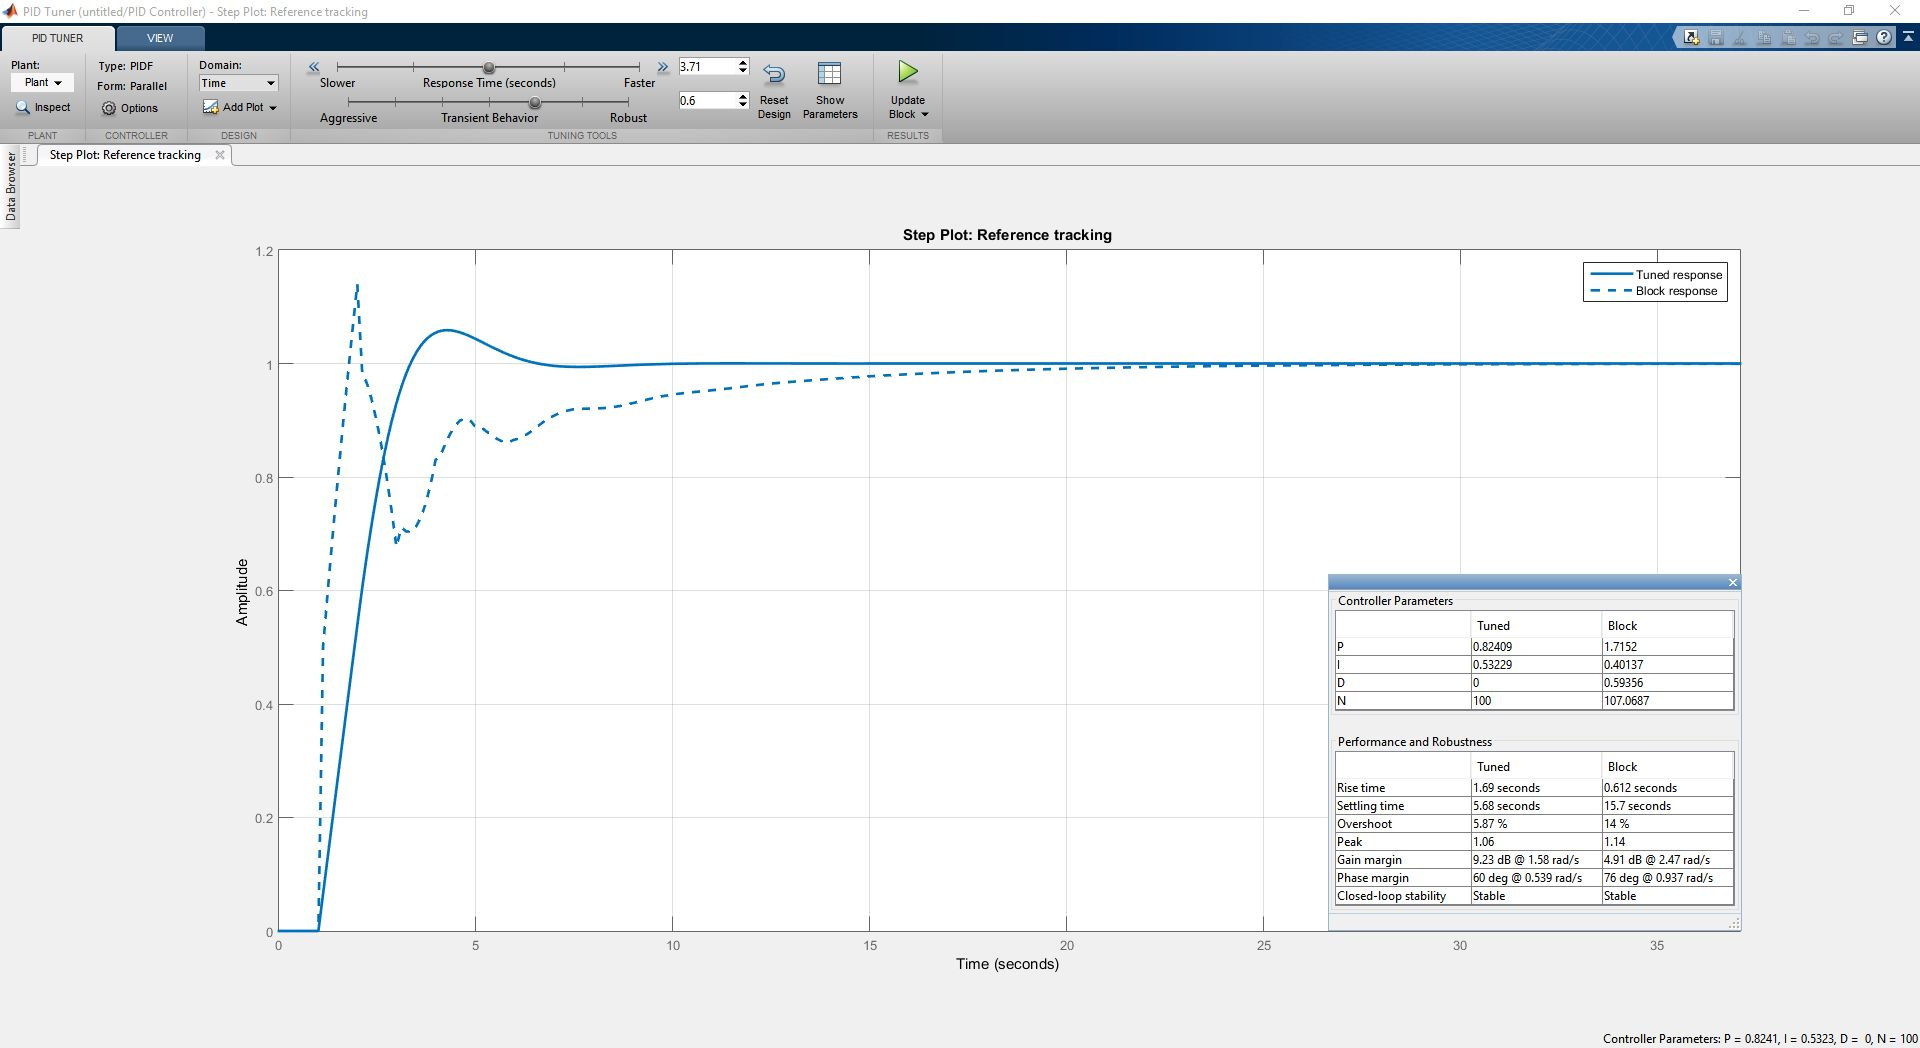
\includegraphics[width=160mm]{PID_Tuner}
	\caption{Zrzut ekranu przedstawiający narzędzie PID Tuner}
	\label{fig:PID_Tuner}
\end{figure}

\noindent Otwiera się wówczas okno, które bazując na podanym modelu wyświetla jego aktualną odpowiedź. Użytkownik jest w stanie zmienić typ regulatora, domyślnie pozostając przy PID. Korzystając z suwaków, można modyfikować czas reakcji oraz agresywność odpowiedzi. Podczas takich zmian, użytkownik na bieżąco obserwuje odpowiedź układu oraz zmieniające się parametry regulatora.
Możliwe jest również wyświetlenie innych przebiegów - takich, jak odpowiedź układu otwartego, odpowiedź skokowa obiektu regulacji - w dziedzinie czasowej lub częstotliwościowej.


